\documentclass[conference]{IEEEtran}
\IEEEoverridecommandlockouts
% The preceding line is only needed to identify funding in the first footnote. If that is unneeded, please comment it out.
\usepackage{cite}
\usepackage{amsmath,amssymb,amsfonts}
\usepackage{algorithmic}
\usepackage{graphicx}
\usepackage{textcomp}
\usepackage{xcolor}
\def\BibTeX{{\rm B\kern-.05em{\sc i\kern-.025em b}\kern-.08em
    T\kern-.1667em\lower.7ex\hbox{E}\kern-.125emX}}
\begin{document}

\title{
    CS 677 Project Proposal: Defect Detection in Semiconductor Wafers Using Image Classification
}

% Authors 
\author{
    \IEEEauthorblockN{Ian S. Jackson}
    \IEEEauthorblockA{\textit{Lane Department of Computer Science and Electrical Engineering} \\
    \textit{West Virginia University}\\
            Morgantown, United States \\
            isj0001@mix.wvu.edu}
}

\maketitle

\section{Introduction}
In the semiconductor manufacturing industry, defect detection is a critical process that directly impacts production yield and device reliability. 
Traditional inspection methods often rely on manual analysis or rule-based systems, which can be time-consuming and prone to human error. 
With advancements in machine learning and computer vision, automated defect detection using image classification techniques offers a more efficient and accurate solution. 
This project aims to develop a machine learning model capable of classifying semiconductor wafer images into various defect categories.

\section{Objective}
The objective of this project is to develop a machine learning model capable of classifying wafer images into different defect categories. 
By leveraging image classification techniques, the system can automate the defect detection process and provide insights into common failure modes.

This project aims to deliver:
A trained and validated machine learning model capable of accurately classifying semiconductor wafer defects,
visualizations of correctly classified and misclassified images, and
a comprehensive report summarizing the methodology, results, and recommendations for further enhancements.

\subsection{Dataset} 
The targeted dataset for this project is the WM-811K Wafer Map Dataset \cite{b1}. 
The dataset contains 811,457 wafer maps collected from 46,393 lots in real-world fabrication, with defect types of: Center, Donut, Edge-Loc, Edge-Ring, Loc, Random, Scratch, Near-full, and none.
Around 20\% of the dataset was annotated by experts \cite{b2}.
% A sample defective wafer can be seen in Figure \ref{fig:ex-data} where green pixels represent a defective chip. 

% \begin{figure}[!ht]
%     \centering
%     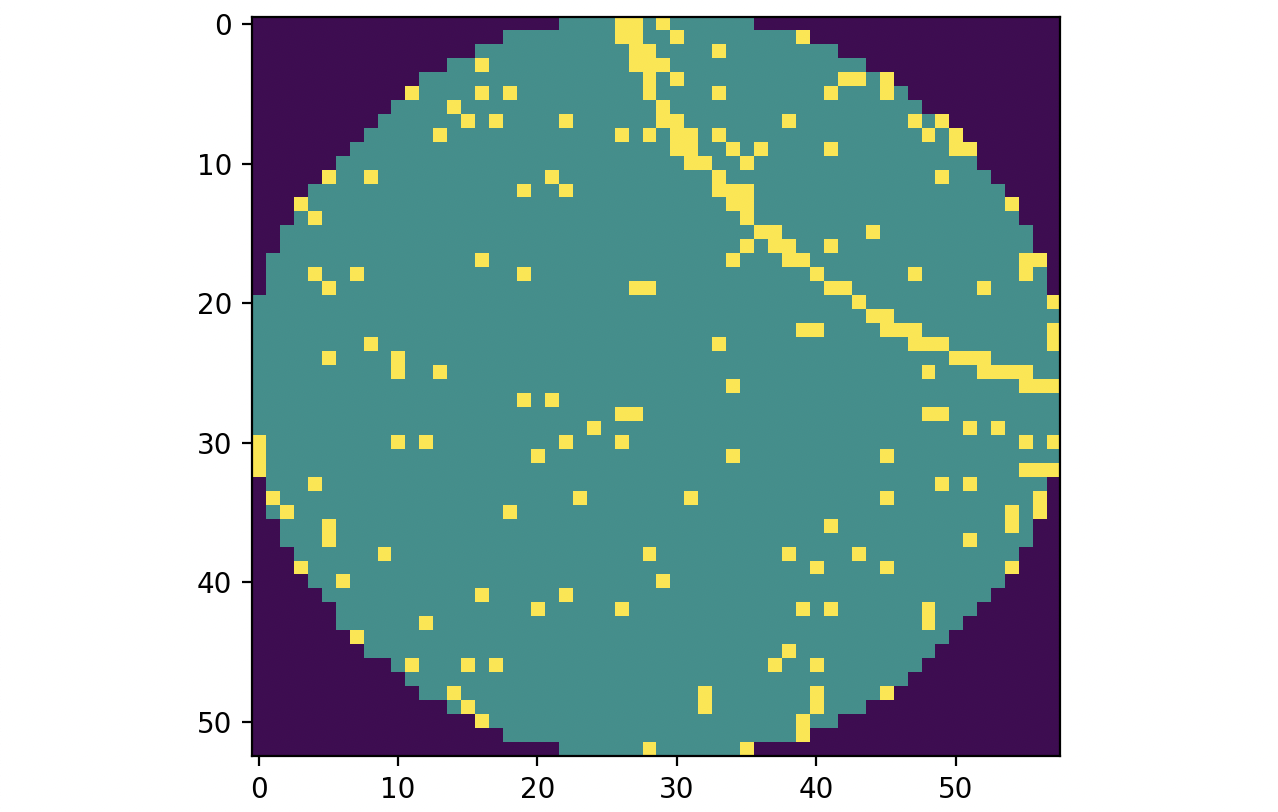
\includegraphics[width=0.75\linewidth]{test1.png}
%     \label{fig:ex-data}
%     \caption{Example Wafer Defect Image from WM-811K Dataset}
% \end{figure}

\section{Model Development} 
The project will use CNNs to extract features and classify defects. As well as, experiment with alternative models such as support vector machines (SVMs) or decision trees with manually extracted image features.
The model will be evaluated by metrics such as accuracy, precision, recall, and F1-score to evaluate model performance.

A reasonable goal for this project is to achieve at least 90\% accuracy in wafer defect classification. 
We also aim for an F1-score of at least 85\% across all defect classes, ensuring that the model performs well even on less frequently occurring defect types. 
Additionally, inference time should remain within an acceptable range (e.g., under 100 milliseconds per image) to facilitate real-time defect detection in a production environment.

\begin{table}[h]
    \centering
    \caption{Project Timeline}
    \begin{tabular}{|c|l|}
    \hline
    \textbf{Week} & \textbf{Main Objective} \\ \hline
    1 & Project Planning \& Literature Review \\ \hline
    2 & Dataset Preparation \& Preprocessing \\ \hline
    3 & Baseline Model Development \\ \hline
    4 & Model Architecture Optimization \\ \hline
    5 & Alternative Model Exploration \\ \hline
    6 & Model Evaluation \& Performance Tuning \\ \hline
    7 & Deployment \& Testing \\ \hline
    8 & Final Model Validation \& Comparison \\ \hline
    9 & Report Writing \& Visualization \\ \hline
    10 & Final Presentation \& Submission \\ \hline
    \end{tabular}
    \label{tab:project_timeline}
\end{table}

\section{Conclusion}
This project aims to leverage machine learning and image classification techniques to enhance defect detection in semiconductor wafer manufacturing. 
The evaluation process will focus on key performance metrics, including accuracy, precision, recall, and F1-score, with a target of at least 90\% accuracy and an F1-score of 85\% or higher. 
Additionally, inference time constraints will be considered to ensure feasibility for real-time applications in semiconductor fabrication environments.

Through this project, we aim to demonstrate the potential of deep learning for improving efficiency and reliability in defect detection. 
The results will be documented in a comprehensive report, providing an analysis of model performance, visualization of classifications and misclassifications, and recommendations for future improvements. 

\begin{thebibliography}{00}
\bibitem{b1} Q. Yi, "WM811K Wafer Map Dataset," Kaggle, 2020. Available: https://www.kaggle.com/datasets/qingyi/wm811k-wafer-map. [Accessed: Jan. 28, 2025].
\bibitem{b2} M. -J. Wu, J. -S. R. Jang and J. -L. Chen, "Wafer Map Failure Pattern Recognition and Similarity Ranking for Large-Scale Data Sets," in IEEE Transactions on Semiconductor Manufacturing, vol. 28, no. 1, pp. 1-12, Feb. 2015, doi: 10.1109/TSM.2014.2364237. [Accessed: Feb. 10, 2025].
\end{thebibliography}
\end{document}
